\documentclass[12pt, a4paper]{report}

\usepackage[utf8]{inputenc}
\usepackage{amsfonts, amssymb, amsmath}
\usepackage{csquotes}
\usepackage[english]{babel}
\usepackage{newlfont}
\usepackage{color}
\textwidth=450pt\oddsidemargin=0pt
\usepackage[top=3cm, bottom=3.5cm,left=2.5cm, right=2.5cm]{geometry}
\usepackage{graphicx}
\usepackage{float}
\usepackage{comment}
\usepackage{caption}
\usepackage{subcaption}
\usepackage[labelformat=empty]{caption}
\usepackage{float}
\usepackage[separate-uncertainty=true]{siunitx}
\usepackage[style=numeric,backend=biber, sorting=none]{biblatex}
\usepackage{titlesec}
\usepackage{dsfont}
\usepackage{listings}
\usepackage[colorlinks=true, linkcolor=blue, urlcolor=cyan, citecolor=green]{hyperref}
\usepackage{cleveref}
\usepackage{xcolor}
\usepackage{xparse}
\usepackage{siunitx}

\addbibresource{thesis.bib}

\numberwithin{equation}{section}

\parindent=0pt

\title{Thesis}
\author{Samuele De Amicis}

\begin{document}

\maketitle

\chapter{Froehlich Polaron}
\section{Electrons in crystals}
The study of electrons inside a solid crystal is an important field due to their role in the determination of transport
and optical properties of such materials.\\
Multiple experiments involving X-ray or electron scattering from suitable solid samples have demonstrated that a crystalline solid, 
whether a metal, an insulator or a semiconductor, is described a periodic arrangement of atoms consisting of a unit cell 
(usually the primitive one, defined as the smallest unit cell possible in a determined material) with a suitable 
atomic basis: some examples are Iron (Fe), described by a BCC (Body-Centered Cubic) unit cell with a single Fe atom basis, 
rock salt (NaCl), described by by a FCC (Face-Centered Cubic) unit cell with a basis composed of one Na atom and one Cl atom, and 
crystalline silicon (Si), which is characterized by the diamond structure, an FCC structure with a basis composed of 2 silicon atoms 
(geometrically different from that seen in rock salt). \\
Given the periodic nature of crystal structures, it is natural to consider the electrostatic potential generated by the crystal to 
be periodic too. Such is the basic assumption which underlies the treatment of electrons in crystals, that was first described by 
Felix Bloch in his famous 1928 paper \textit{Uber die Quantenmechanikder Elektronen in Kristallgittern} \cite{bloch1928quantum}.\\
The model proposed by Bloch assumed independent electrons (no electron-electron interactions terms): each electron behaves as 
if only an average contribution to the potential from the other electrons (with the same periodicity of the lattice) exists, thus 
retrieving an \textbf{effective one-electron potential}.\\
The resulting Hamiltonian for the single independent electron is:
\begin{equation}
    \mathrm{H}\psi(r)=\left(-\frac{\hbar^2}{2m}\nabla^2+V(r)\right)\psi(r)=E\psi(r),
    \label{eq_0_00}
\end{equation}
where $V(r)$ is a periodic potential with the lattice periodicity, given a lattice translation vector
\begin{equation}
    \mathbf{T}=n_1\mathbf{a_1}+n_2\mathbf{a_2}+n_3\mathbf{a_3},\hspace{1cm}n_1,n_2,n_3\hspace{0.5cm}\mathrm{integers},
\end{equation}
with $\mathbf{a_1}$, $\mathbf{a_2}$ and $\mathbf{a_3}$ primitive translation vectors.
Therefore, we have
\begin{equation}
    V(r+T)=V(r)
\end{equation}
This means that the potential can be expanded in Fourier series
\begin{equation}
    V(r)=\sum_KV_Ke^{iK\cdot r},
\end{equation}
and is consequently useful to expand the wavefunction in the same way. For this reason the Born-von Karman boundary conditions
are applied \cite{Ashcroft76}
\begin{equation}
    \psi(r+N_ia_i)=\psi(r),\hspace{1cm}i=1,2,3.
\end{equation}
where $N_ia_i$ is a chosen vector such that $V(r+N_ia_i)=V(r)$ (it is a translation vector for the lattice). This is a normalizing
condition for the wavefunction which corresponds to taking $N_i$ unit cell in each direction and periodically repeating them. In this 
way it is possible to write the wavefunction in the following way:
\begin{equation}
    \psi(r)=\sum_qc_qe^{iq\cdot r}.
    \label{eq_0_01}
\end{equation}
Going back to the periodic potential $U(r)$ we observe that the Fourier terms $U_K$ are related to $U(r)$ by
\begin{equation}
    U_K=\frac{1}{v}\int_{cell}dre^{-iK\cdot r}U(r)
\end{equation}
with $v$ unit cell volume and $K$ reciprocal lattice vector (vector in k-space such that $e^{iK\cdot a_i}=1$). If it is 
assumed that the potential $V(r)$ is real and $V(-r)=V(r)$ (valid for every Bravais lattice) it follows that the coefficients 
$U_K$ are real.\\
Substituting in \ref{eq_0_00} we obtain:
\begin{equation}
    (\mathrm{H}-E)\psi(r)=\sum_q\left(\frac{\hbar^2}{2m}q^2-E\right)c_qe^{iq\cdot r}+\sum_{Kq'}U_Kc_{q'-K}e^{iq'\cdot r}=0,
\end{equation}
which yields the following result:
\begin{equation}
    \left(\frac{\hbar^2}{2m}(k-K)^2-E\right)c_{k-K}+\sum_{K'}c_{K'-K}c_{k-K'}=0.
\end{equation}
From this equation it becomes clear that for a fixed $k$ only the coefficients $c_k,c_{k-K},...$ whose wavevector differs from 
$k$ by a reciprocal lattice vector are coupled. In this way the original problem has been divided in $N$ independent equations for 
each allowed value of $k$ (in the first Brillouin zone, the primitive unit cell in the reciprocal space).\\
Going back to the expansion \ref{eq_0_01} the wavefunction now becomes:
\begin{equation}
    \psi_k(r)=\sum_{K}c_{k-K}e^{i(k-K)\cdot r},
\end{equation}
which can be recast as 
\begin{equation}
    \psi_k(r)=e^{ik\cdot r}\sum_{K}c_{k-K}e^{-iK\cdot R};
\end{equation}
in this form it is easy to recognize that 
\begin{equation}
    u_k(r)=\sum_Kc_{k-K}e^{-iK\cdot R}
\end{equation}
has the periodicity of the (reciprocal) Bravais lattice.\\
The shape of the Bloch wavefunction as stated in the Bloch theorem is thus retrieved
\begin{equation}
    \psi_k(r)=e^{ik\cdot r}u_k(r)
\end{equation}
and its square modulus (from which important properties such as charge distribution follow) $|\psi(k)|^2$ has the periodicity of the
lattice.\\
The new Hamiltonian eigenvalues equation using Bloch wavefunction reads
\begin{equation}
    \mathrm{H}_k u_{nk}=\left(\frac{\hbar^2}{2m}\left(\frac{1}{i}\nabla+k\right)^2+U(r)\right)u_{nk}(r)=E_{nk}u_{nk}(r),
\end{equation}
which yields a different energy eigenvalue for each $k$ in the first Brillouin zone. The index $n$ arises from the fact that for 
each $k$ value infinite discrete solutions to the eigenvalue equation exist, in the same as in the particle in a box problem. Going 
to the thermodynamic limit ($N_i\to\infty$ for each component $i$) the entire first Brillouin zone is sampled and the typical band 
structure of the solids is recovered.\\
All the methods employed in solid state calculations rely on this "simple" equation to determine band structures, granted 
analytical form of the periodic potential $U(r)$ can be retrieved.\\
The most used and effective computation method is \textbf{Density Functional Theory} \cite{thijssen2007computational} or \textbf{DFT} 
for short, which does not directly compute the eigenvalue equation for each single $k$ and $n$ value, which would be impossible since 
the potential $U(r)$ is a many-body object that includes electron-electon interactions, but rather computes all the physical quantities of 
interest starting from the ground state charge density $\rho_0(r)$. This is made possible by the two Hohenberg-Kohn theorems \cite{hohenberg1964inhomogeneous}, 
which respectively state that the external potential (the periodic $U(r)$ from the electron point of view) is uniquely determined 
up to a constant by the ground state charge density $\rho_0(r)$ and that this density can be computed variationally by minimizing a suitable 
functional $F[\rho]$.\\
Nevertheless, the functional $F[n]$ exact form is unknown: for this reason the \textbf{Kohn-Sham scheme} \cite{PhysRev.140.A1133} 
is used. The idea at the basis of this practical setup is to substitute the real interacting system (many-body) with an auxiliary non-interacting
one (single particle) which has the same ground state as the original. In this system the total potential $V(r)=V_{ion}(r)+V_{ee}(r)$ is 
replaced with an effective potential $V_{eff}(r)$ defined as
\begin{equation}
    U_{eff}(r)=U_{ion}(r)+U_H(r)+U_{xc}(r),
\end{equation}
where $U_{ion}$ is the ionic potential, often modelled using pseudopotentials \cite{kerker1980non}, $U_H(r)$ is the Hartree term, the electrostatic 
potential due to the mean field distribution of all the other electrons, and $U_{xc}$ the exchange-correlation term, an approximate potential 
which includes Pauli exclusion principle (exchange), higher order electron-electron interactions (correlation) and many body corrections to kinetic energy. The exchange-correlation 
term is usually computed using \textbf{LDA} (Local Density Approximation) or \textbf{GGA} (Generalized Gradient Approximation), both based on the the Uniform Electron 
Gas (UEG) \cite{ziesche1998density}.
Despite the inevitable approximations, DFT calculations are able to provide extremely accurate band structure calculations 
with few drawbacks, such as inaccurate gap estimations in insulators and semiconductors.
\begin{figure}[H]
    \centering
    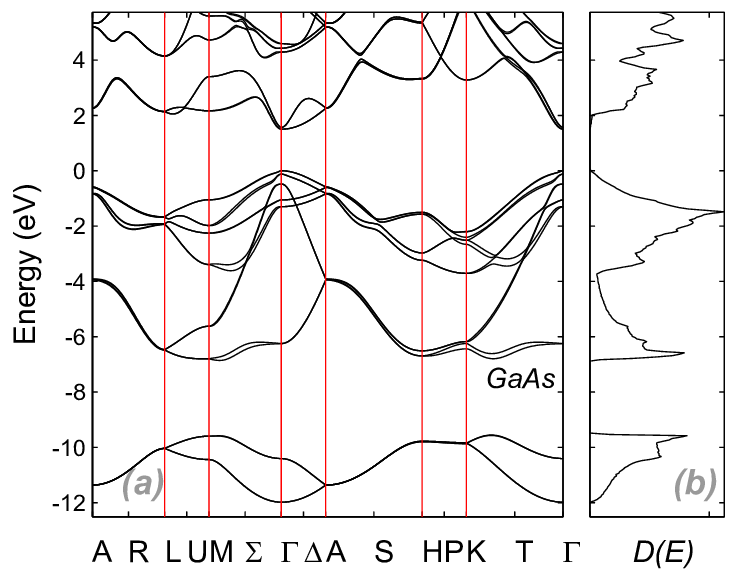
\includegraphics[scale=0.4]{a-Calculated-low-temperature-band-structure-for-GaAs-in-WZ-phase-b-Calculated-DOS.png}
    \caption{DFT calculated low-temperature GaAs Wurtzite structure with relative DOS \cite{GaAs_wurtzite_structure}}
    \label{fig:GaAs_Wurtzite_structure}
\end{figure}
As it can be seen in Figure \ref{fig:GaAs_Wurtzite_structure} for GaAs, at the band extrema (at the edge between the allowed band states 
and the forbidden gap) the bands have a quadratic dispersion akin to that of a free electron: an electron in these regions only feel a 
very weak external potential $U(r)$ and can be considered as free provided that the free electron mass $m$ is substituted with an effective mass 
$m^*$ which takes into account the potential acting on it.\\
In a general case the effective mass is a tensorial quantity (bands are anisotropic in general with respect to the wavevector) and 
their value can be computed with
\begin{equation}
    m^{*-1}_{ij}=\frac{1}{\hbar^2}\frac{\partial^2 E}{\partial k_i \partial k_j},
    \label{eq_effective_mass}
\end{equation}
provided that the quadratic approximation is valid. This approximation is really useful when calculating quantities near band extrema, 
providing an effective description of an otherwise complex interaction.
\section{The polaron problem: the Froehlich model}
The treatment described up until now for electrons in solids relies on a basic assumption: electro dynamics is much faster than ion 
dynamics. This is the so-called \textbf{Born-Oppenheimer approximation}, which assumes that the motion of the much heavier ions is 
slow compared to the fast dynamics of the electrons (the characteristic time are of the order of $ps$ for ions and $fs$ for 
electrons). As a result, electrons are considered to respond instantaneously to changes in the positions of the ions, allowing 
the separation of electronic and ionic degrees of freedom in the analysis. Given $M$ ions and $n$ electrons the wavefunction 
$\Psi(R_1,...,R_M,r_1,...,r_n)$ with $R_\alpha$ ionic positions and $r_i$ electron positions can be decomposed in the following way:
\begin{equation}
    \Psi(R_1,...,R_M,r_1,...,r_n)=\chi(R_1,...,R_M)\psi(r_1,...,r_n),
\end{equation}
and only the electronic wavefunction $\psi(r_1,...,r_n)$ is taken into consideration, decoupling ionic degrees of freedom and treating 
ionic potential as a constant energy surface $U_{ion}(r)$.\\
This approximation, although extremely effective in computing electronic bands, fails by design to describe systems where there is a 
strong coupling between electrons and ions (for example electron-phonon interaction).\\
Such is the case of polar crystals: in these materials single electrons at the bottom of the conduction band (or holes at the top of 
the valence band) couple to the strongly polarized ions and distort the unit cell: an electron-phonon interaction is thus present 
in the lattice and the electron properties (such as energy and effective mass) are renormalized due to this coupling \cite{frohlich1954electrons}.\\
The basic assumption of the Froehlich model is that the polaron is "large", namely the characteristic size of the polaron (electron together 
with its phonon cloud) is much larger than the lattice constant $a$. In this way it is possible to ignore the atomic details of the actual 
material and treat it as a uniform dielectric medium.\\
It is assumed that the electron which takes part in the formation of the polaron lies at the bottom of the valence band, in this way it is 
expected to have a quadratic energy dispersion characterized (as already seen in \ref{eq_effective_mass}) by an effective mass
\begin{equation}
    \epsilon(k)=\frac{\hbar^2k^2}{2m^*},
\end{equation}
where the effective mass $m^*$ encapsulates all the interactions due to crystal structure (for a hole polaron the dispersion is similar 
considering a negative effective mass).\\
Given the fact that we are dealing with the large polaron model, it is possible to treat the material as an homogeneous continuum 
which is polarized by the excess charge (the conduction electron). We also assume that the material is isotropic.
Let $P(r)$ be the electric polarization at the point $r$, the total electric field is then:
\begin{equation}
\begin{split}
    &D(r)=\epsilon_0E(r)+4\pi P(r),\\
    &D(r)=\epsilon E(r).
\end{split}
\end{equation} 
The only free charge present in the material is the conduction electron in excess, this means that $D(r)$ is completely determined by it:
\begin{equation}
\begin{split}
    &D(r,r_{el})=-\nabla\frac{e}{|r-r_{el}|}, \\
    &\nabla\cdot D(r,r_{el})=4\pi\delta(r-r_{el}),
\end{split}
\end{equation}
with $r_{el}$ the coordinate of the conduction electron. Developing the equations the following relation is obtained:
\begin{equation}
    4\pi P(r) = \left(1-\frac{1}{\epsilon}\right)D(r).
\end{equation}
$P(r)$ is the total polarization, which has the contribution both from electrons and from ionic displacements, since only the second 
contribution is relevant in our treatment, a method to tell apart this two contributions is needed.\\
To obtain this we imagine a system where a field is slowly applied and then rapidly switched off \cite{haken1976quantum}: only 
electrons are able to keep up with the variation of the field. A formula connecting polarization and $D$ (dropping the $r$ dependence 
since an isotropic and homogeneous medium is assumed) is then retrieved as
\begin{equation}
    4\pi \delta P = -\left(1-\frac{1}{\epsilon_\infty}\right)D,
\end{equation}
it is then obtained the lattice contribution to the polarization:
\begin{equation}
    4\pi P_{lat} = 4\pi(P-\delta P) = \left(\frac{1}{\epsilon_\infty}-\frac{1}{\epsilon_0}\right)D.
    \label{eq_polarization_lattice}
\end{equation}
We know consider a model for the polar crystal lattice: we assume it to be constituted of individual oscillating discrete dipoles 
located at fixed sites of the crystal with characteristic frequency $\omega$. The energy of each one of these oscillators is 
\begin{equation}
    \frac{M}{2}(\dot{q}^2+\omega^2q^2).
\end{equation}
The next step is to move from a discrete set of fixed oscillators to a continuum of dipoles: it is assumed that the dipoles are not 
coupled. Defining the effective charge as $e^*$, the following substitution is made:
\begin{equation}
    e^*q_n\to \mathbf{P}_{lat}(r),
\end{equation}
which relates the dipole moment to the polarization field. We also write the following relation:
\begin{equation}
    \frac{M}{e^{*2}}=\gamma d^3r,
\end{equation}
where $M=nd^3r$ is the mass density of the medium.\\
It is now possible to define the kinetic and potential energy of the freely oscillating polarization field:
\begin{equation}
\begin{split}
    &T=\int \frac{\gamma}{2}\dot{\mathbf{P}}_{lat}^2(\mathbf{r})d^3r,\\
    &V=\int \frac{\gamma\omega^2}{2}\mathbf{P}_{lat}^2(\mathbf{r})d^3r.
\end{split}
\end{equation}
We identify $\omega$ with the optical phonon frequency $\omega_{LO}$, but the constant $\gamma$ has not yet been given a physical 
definition. For this reason we consider the interaction between electrons and dipole moment, which is given by 
\begin{equation}
    e\frac{\mathbf{r}-\mathbf{r}'}{|\mathbf{r}-\mathbf{r}'|^3}\mathbf{P}_{lat},
\end{equation}
which, using a continuous charge distribution and the polarization field, becomes
\begin{equation}
    \rho(\mathbf{r})d^3r\frac{\mathbf{r}-\mathbf{r}'}{|\mathbf{r}-\mathbf{r}'|^3}\mathbf{P}_{lat}(\mathbf{r}')d^3r'.
\end{equation}
The interaction energy $E_I$ is thus
\begin{equation}
    E_I=\iint \rho(\mathbf{r})\frac{\mathbf{r}-\mathbf{r}'}{|\mathbf{r}-\mathbf{r}'|^3}\mathbf{P}_{lat}(\mathbf{r}')d^3rd^3r'.
\end{equation}
The Lagrangian is then built as follows:
\begin{equation}
    L=T-U-E_I
\end{equation}
and the equation of motion are found solving the Lagrange equations
\begin{equation}
    \frac{d}{dt}\frac{\delta L}{\delta \dot{P}_{lat_i}}-\frac{\delta L}{\delta P_{lat_i}}=0
\end{equation}
for $i=1,2,3$. The explicit formula of the equation of motion is:
\begin{equation}
    \gamma(\ddot{\mathbf{P}}_{lat}(\mathbf{r}')+\omega^2\mathbf{P}_{lat}(\mathbf{r}'))=-\int \frac{\mathbf{r}-\mathbf{r}'}{|\mathbf{r}-\mathbf{r'}|^3}\rho(\mathbf{r})d^3r
\end{equation}
keeping fixed $\rho(\mathbf{r})$. The term on the right side is simply the dielectric displacement $\mathbf{D}(\mathbf{r}')$ and, in the 
static limit, the equation simplifies to
\begin{equation}
    \gamma\omega^2\mathbf{P}_{lat}(\mathbf{r}')=\mathbf{D}(\mathbf{r}').
\end{equation}
Comparing this equation with \ref{eq_polarization_lattice}, the value of $\gamma$ is obtained:
\begin{equation}
    \gamma = \frac{4\pi}{\omega^2}\left(\frac{1}{\epsilon_\infty-\frac{1}{\epsilon_0}}\right)^{-1}.
\end{equation}
It is now time to define the full complete polaron Hamiltonian. We start by defining the free electron term (the interaction lies inside 
the effective mass $m^*$), considering that the electron charge density operator is defined as:
\begin{equation}
    \rho(\mathbf{r})=-e\psi^\dagger(\mathbf{r})\psi(\mathbf{r})
\end{equation}
using the second quantization formalism with field operators, then the electron kinetic term is
\begin{equation}
    H_{el}=\int\psi^\dagger(\mathbf{r})\left(-\frac{\hbar^2}{2m^*}\nabla^2\right)\psi(\mathbf{r})d^3r.
    \label{el_kinetic_hamiltonian_r_formalism}
\end{equation}
If we use a suitable basis for the field operator
\begin{equation}
    \psi(\mathbf{r})=\frac{1}{\sqrt{V}}\sum_\mathbf{k}c_\mathbf{k}e^{i\mathbf{k}\cdot\mathbf{r}}
\end{equation}
with $V$ (unit cell) volume, then \ref{el_kinetic_hamiltonian_r_formalism} becomes
\begin{equation}
    H_{el}=\sum_\mathbf{k}\frac{k^2}{2m^*}c^\dagger_\mathbf{k}c_\mathbf{k},
    \label{el_kinetic_hamiltonian_k_formalism}
\end{equation}
with $c^\dagger_\mathbf{k}$ and $c_\mathbf{k}$ creation and annihilation operators for the free electron.\\
We now turn our attention to the polarization field, taking into account that it can be modelled as an harmonic oscillator a 
form similar to \ref{el_kinetic_hamiltonian_r_formalism} can be recovered ($P_{lat}$ is substituted by $P$ in the following equations):
\begin{equation}
    H_{ph}=\int\left(\frac{1}{2\gamma}\mathbf{\Pi}^2(\mathbf{r})+\frac{\gamma}{2}\omega^2\mathbf{P}^2(\mathbf{r})\right)d^3r,
\end{equation}
where $\mathbf{\Pi}(\mathbf{r})$ is the conjugate momentum to $\mathbf{P}(\mathbf{r})$.\\
Using the canonical substitution for the operator $\mathbf{P}(\mathbf{r})$ 
\begin{equation}
    \mathbf{P}(\mathbf{r})=\frac{1}{\sqrt{V}}\sum_{\mathbf{q}}\sqrt{\frac{\hbar}{2\gamma\omega}}\frac{\mathbf{q}}{q}e^{i\mathbf{q}\cdot\mathbf{r}}(a_\mathbf{q}-a_\mathbf{-q}^\dagger)
\end{equation}
and the corresponding one for $\mathbf{\Pi}(\mathbf{r})$ we obtain the equation for a quantum harmonic oscillator:
\begin{equation}
    H_{ph}=\hbar\omega\sum_\mathbf{q} a^\dagger_\mathbf{q}a_\mathbf{q}
\end{equation}

The Froehlich model provides a quantum mechanical description of this phenomenon, focusing on the interaction between an electron 
and the longitudinal optical (LO) phonons in an ionic crystal. The Froehlich Hamiltonian is given by:
\begin{equation}
    H = \frac{p^2}{2m^*} + \sum_{\mathbf{q}} \hbar \omega_{LO} a^\dagger_{\mathbf{q}} a_{\mathbf{q}} + \sum_{\mathbf{q}} \left( V_{\mathbf{q}} e^{i\mathbf{q}\cdot\mathbf{r}} a_{\mathbf{q}} + V^*_{\mathbf{q}} e^{-i\mathbf{q}\cdot\mathbf{r}} a^\dagger_{\mathbf{q}} \right),
\end{equation}
where $p$ is the electron momentum, $m^*$ is the effective mass, $a^\dagger_{\mathbf{q}}$ and $a_{\mathbf{q}}$ are the creation and annihilation operators for LO phonons of wavevector $\mathbf{q}$ and frequency $\omega_{LO}$, and $V_{\mathbf{q}}$ describes the electron-phonon coupling strength.

This model captures the essential physics of large polarons, where the electron is dressed by a cloud of virtual phonons, leading to a renormalization of its mass and mobility. The strength of the electron-phonon interaction is characterized by the dimensionless Froehlich coupling constant $\alpha$, which determines the degree of polaronic effects in the material.
\printbibliography
\end{document}